	\documentclass[a4paper]{article}
	
	\usepackage[portuguese]{babel}
	\usepackage[utf8]{inputenc}
	\usepackage{indentfirst}
	\usepackage{graphicx}
	\usepackage{verbatim}
	\usepackage{wrapfig, blindtext}
	\usepackage{listings}
	\usepackage{textcomp}
	\usepackage{color}
	\usepackage{xcolor}
	\usepackage[left=1in,right=1in,top=1in,bottom=.8in]{geometry}
	\usepackage{float}

\graphicspath{ {res/} }

	%%%%%%%%%%% CONFIGURATION OF CODE INPUT %%%%%%%%%%%%%%%%%%%%%%
\lstset{
  language=C,
  tabsize=4,
  captionpos=b,
  numbers=left,
  frame=single,
  breaklines=true,
  rulecolor=\color{black},
  title=Struct linkLayer,
  commentstyle=\color{codeGreen},
  backgroundcolor=\color{codeBackground},
  numberstyle=\color{gray},
  keywordstyle=\color{blue} \textbf,%otherkeywords={xdata},
  keywords=[2]{xdata},
  keywordstyle=[2]\color{red}\textbf,
  identifierstyle=\color{black},
  stringstyle=\color{red}\ttfamily,
  basicstyle = \ttfamily \color{black} \footnotesize,
  showstringspaces=false ,
}
%%%%%%%%%%%%%%%%%%%%%%%%%%%%%%%%%%%%%%%%%%%%%%%%%%

	\begin{document}
	

\definecolor{codeBackground}{RGB}{220, 220, 220}
\definecolor{codeGreen}{RGB}{0, 150, 0}
	\setlength{\textwidth}{16cm}
	\setlength{\textheight}{22cm}
	
	\title{\Huge\textbf{Lab 2}\linebreak\linebreak\linebreak
	\Large\textbf{Relatório Final}\linebreak\linebreak
	\linebreak\linebreak
	
\includegraphics[scale=0.1]{./res/feup-logo.png}\linebreak\linebreak
	\linebreak\linebreak
	\Large{Mestrado Integrado em Engenharia Informática e Computação} \linebreak\linebreak
	\Large{Redes de Computadores}\linebreak
		}
	

	\author{
	\textbf{Grupo 3:}\\
	Francisco Rodrigues - 201305627 \\
	João Nogueira - up201303882 \\
	Marta Lopes - 201208067 \\
	\linebreak\linebreak \\
	 \\ Faculdade de Engenharia da Universidade do Porto \\ Rua Roberto Frias, s\/n, 4200-465 Porto, Portugal \linebreak\linebreak\linebreak
	\linebreak\linebreak\vspace{1cm}}
	
	\maketitle
	\thispagestyle{empty}

	\newpage

	\section{Sumário}
	\normalsize

Este relatório tem como objetivo explicar o segundo projeto da Unidade Curricular de Redes de Computadores bem como analisar os resultados obtidos na realização das experiências especificadas no enunciado do mesmo.

	\newpage

	\tableofcontents	

	\newpage

	\section{Introdução}

	Este projeto encontra-se dividido em duas grandes partes. Em primeiro lugar, é-nos pedido que desenvolvamos uma aplicação de \textit{download} que proceda à transferência de um ficheiro e que implemente o protocolo \textit{FTP}. Em segundo lugar, é-nos pedido que configuremos e estudemos uma Rede de Computadores seguindo a estrutura das experiências abaixo enumeradas:

\begin{enumerate}

\item Configuração de um \textit{IP} de rede;
\item Configuração de duas Redes \textit{LAN} virtuais num \textit{switch};
\item Configuração de um \textit{router} em \textit{Linux};
\item Configuração de um \textit{router} comercial implementando \textit{NAT};
\item \textit{DNS};
\item Conexões \textit{TCP}.

\end{enumerate}

	\section{Parte 1 - Aplicação de download}

	Como referido anteriormente, a primeira parte deste tranalho consiste numa aplicação que transfere um ficheiro utilizando o protocolo \textit{FTP} descrito no ficheiro RFC959. Como método de \textit{input} é utilizada a sintaxe mostrada na figura abaixo como descrito no ficheiro RFC1738.

	\begin{figure}[H]
  	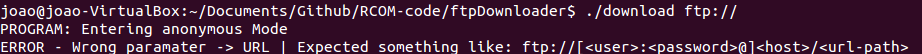
\includegraphics[width=\linewidth]{consoleScreenshot1.png}
  	\caption{Input}
  	\label{fig:input}
	\end{figure}

	A aplicação desenvolvida permite que seja feito um download em modo anónimo. Para tal basta não colocar os caracteres '@' e ':' e não colocar nome de utilizador e password. Neste caso a aplicação irá assumir o utilizador \textit{anonymous} e a palavra-passe vazia.

	\subsection{Arquitetura}

	A \textit{UrlStruct} é a estrutura definida respponsável por guardar a informação necessária que depende do \textit{input} do utilizador.

	\lstset{basicstyle=\ttfamily \color{black}\tiny, title=urlStruct}
	\lstinputlisting{./res/res1.c}
	\normalsize

	Ao correr o programa é chamada a função \textit{getUrlInfo} que é responsável por pegar na \textit{string} que o utilizador forneceu como argumento e interpretar toda a informação necessária.

	\lstset{basicstyle=\ttfamily \color{black}\tiny, title=Url Header}
	\lstinputlisting{../ftpDownloader/url.h}
	\normalsize

	Depois de interpretar a informação introduzida pelo utilizador, e após verificar que esta informação é válida é chamada a função \textit{startConection} responsável por ligar o cliente \textit{FTP} ao servidor através de um \textit{socket}. Com a ligação estabelecida é então necessário chamar função \textit{getControl}, responsável por enviar a informação necessária para o \textit{login} e por enviar o comando \textbf{\textit{PASV}}, o que vai permitir que haja comunicação em ambos os sentidos.

	\lstset{basicstyle=\ttfamily \color{black}\tiny, title=getControl}
	\lstinputlisting{./res/res2.c}
	\normalsize

	 É também feita uma nova conexão através da função \textit{startReceiverConection} para permitir a receção do ficheiro. pedido pelo utilizador. Por fim é enviado o comando \textbf{\textit{RETR}} e recebido o ficheiro a ser guardado. A função \textit{receiveFile} é responsável por enviar o comando, receber o ficheiro e escrevê-lo no disco.

	Terminada a receção do ficheiro resta apenas fechar os \textit{sockets} abertos e libertar a memória alocada para terminar o programa.

	As funções acima referidas e outras auxiliares estão definifdas abaixo, bem como nos anexos.

	\lstset{basicstyle=\ttfamily \color{black}\tiny, title=conection.h}
	\lstinputlisting{../ftpDownloader/conection.h}
	\normalsize
	
	Durante o desenvolvimento da aplicação foi implementado um modo de \textit{debug} que é ativo ao alterar a Macro \textit{DEBUG} de 0 para 1. Este modo faz com que haja mais impressões na consola, o que permite controlar com maior exatidão o modo como a aplicação está a funcionar.

	\lstset{basicstyle=\ttfamily \color{black}\tiny, title=Macros}
	\lstinputlisting{./res/res3.c}
	\normalsize

	\subsection{Resultados}

	Esta aplicação foi testada com diversos ficheiros, tanto em modo anónimo como em modo não anónimo. A transferência dos vários ficheiros foi verificada tendo sido o máximo ficheiro testado um ficheiro de vídeo com cerca de 200MB.

	Em caso de erro, para além da aplicação terminar é impresso na consola o erro em causa, de modo a que o utilizador tenha o máximo controlo possível sobre o sucedido.

	\section{Parte 2 - Configuração de Redes}

	\clearpage

	\section{Conclusões}



	%************************************************************************************************
	\newpage

	\section{Anexos}
	
	\subsection{Headers}

	\subsubsection{conection.h}

	\lstset{basicstyle=\ttfamily \color{black}\small,  title=Anexo 1 - conection.h}
	\lstinputlisting{../ftpDownloader/conection.h}

	\subsubsection{url.h}

	\lstset{basicstyle=\ttfamily \color{black}\small,  title=Anexo 2 - url.h}
	\lstinputlisting{../ftpDownloader/url.h}

	\subsubsection{utilities.h}

	\lstset{basicstyle=\ttfamily \color{black}\small,  title=Anexo 3 - utilities.h}
	\lstinputlisting{../ftpDownloader/utilities.h}

	\subsection{*.c files}

	\subsubsection{main.c}

	\lstset{basicstyle=\ttfamily \color{black}\small,  title=Anexo 4 - main.c}
	\lstinputlisting{../ftpDownloader/main.c}

	\subsubsection{conection.c}

	\lstset{basicstyle=\ttfamily \color{black}\small,  title=Anexo 5 - conection.c}
	\lstinputlisting{../ftpDownloader/conection.c}

	\subsubsection{url.c}

	\lstset{basicstyle=\ttfamily \color{black}\small,  title=Anexo 6 - url.c}
	\lstinputlisting{../ftpDownloader/url.c}

	\subsubsection{utilities.c}

	\lstset{basicstyle=\ttfamily \color{black}\small,  title=Anexo 7 - utilities.c}
	\lstinputlisting{../ftpDownloader/utilities.c}

	\subsection{Makefile}

	\lstset{
   	language=[gnu] make,
   	keywordstyle=\color{teal}\textbf,
   	stringstyle=\color{blue},
   	identifierstyle=\itshape,
	title=Anexo 8 - Makefile
	}
	\lstinputlisting{./res/Makefile.txt}

	\end{document}
